\documentclass[french, a4paper, 11pt]{article}
% avec table des matières : remplacer article par report
% Language setting
% Replace `english' with e.g. `spanish' to change the document language
\usepackage[main=french]{babel}
%\date {Écrit le 26 décembre 2022}

% Set page size and margins
% Replace `letterpaper' with `a4paper' for UK/EU standard size
\usepackage[letterpaper,top=2cm,bottom=2cm,left=2cm,right=2cm,marginparwidth=1.75cm]{geometry}

% Useful packages
\usepackage{amsmath}
\usepackage{array}
\usepackage{graphicx}
\usepackage[colorlinks=true, allcolors=blue]{hyperref}
\usepackage{listings}
\lstset{extendedchars=\true}
\usepackage{pythontex}
\usepackage{changepage}
%\setpygmentspygopt{bash}{style=default} %Set syntax highlighting style
%\setpygmentsfv{xleftmargin=4ex} %Pass fancyvrb options, in this case, left margin
\usepackage{csquotes}
\usepackage[backend=biber, style=nature]{biblatex}
\usepackage{hyperref} % Charge le package hyperref

\title{Installation de Windows 10 : trucs et astuces, réglages}

\author{EMBARKI Naël}


\begin{document}
\maketitle
\fbox{%
   \begin{minipage}{0.9\textwidth}
   	\begin{center}
       \textbf{Ce document a pour but de vous guider dans votre installation de Windows, en cas de problème.s rencontré.s. Merci de le LIRE ENTIÈREMENT afin de prendre en compte chaque cas possible selon les problèmes que vous avez déjà rencontrés ainsi que le constructeur de votre PC (ASUS, Acer, Hp, DELL, etc...). Ce document sera fourni au maximum, si suite à cela votre soucis n'est pas réglé, merci de me contacter sur \texttt{discord} en envoyant une demande d'amis à \texttt{naelebk} ou bien de rejoindre mon \href{https://discord.gg/ja7t6Aq}{\color{blue} serveur discord}.}
       \end{center}
   \end{minipage}
}
$ $ \\ \\

\begin{table}[ht]
    \centering
    \begin{tabular}{|c|>{\bfseries}c|>{\bfseries}c|}
        \hline
        \textbf{Constructeur} & \textbf{Touche Boot Menu} & \textbf{Touche BIOS} \\
        \hline
        Acer & F12 & Suppr, F2 \\
        Apple & Option (Alt) & Command + R, Option (Alt) + Command + P + R \\
        ASUS & Echap, F8 & Suppr, F2 \\
        Dell & F12 & F2 \\
        HP & Echap, F9 & Echap, F10, F1 \\
        Lenovo & F12 & F1, F2 \\
        MSI & F11 & Suppr \\
        Sony & F11, Echap, Assist & F1, F2 \\
        Toshiba & F12 & F2 \\
        \hline
    \end{tabular}
    \caption{Touches pour accéder au \texttt{Boot Menu} et au \texttt{BIOS} selon le constructeur.}
    \label{tab:boot-bios-keys}
\end{table}

\section*{0. Intrada}
\noindent Avant toute chose, il est important de créer une clé \texttt{USB} bootable afin d'installer Windows 10/11 sur ce dernier. De préférence, il vous en faudrait une d'au moins \texttt{8 Go} (PS : si vous avez entre 6 et 7 c'est ok). Pour créer une clé \texttt{USB}, vous pouvez soit la créer depuis un autre PC Windows 10 (cas le plus simple si vous avez un autre PC à votre disposition), soit directement depuis Linux si vous n'avez pas un autre PC à votre disposition. Pour Linux, deux options s'offrent à vous pour créer une clé \texttt{USB} : 
\begin{itemize}
    \item En suivant \href{https://www.youtube.com/watch?v=FQl0nLe4erw&ab_channel=Na\%C3\%ABlEBK}{\color{blue} cette vidéo} (solution la plus simple, mais ni la plus rapide, ni la plus pertinente)
    \item Si vous n'arrivez pas à installer WoeUSB pour créer une clé \texttt{USB} bootable, vous pouvez utiliser à la rigueur \texttt{Ventoy} qui est un outil permettant de booter sur plusieurs systèmes d'exploitation différents à partir d'une seule clé \texttt{USB}, synopsis (solution plus rapide, plus complexe et plus pertinente) : \begin{verbatim}
    $ cd ~/Documents
    $ curl -O https://raw.githubusercontent.com/naelebk/useful_scripts/main/ventoy.sh
    // Ici, dans ce répertoire, téléchargez une image ISO de Windows (10/11) 
    // depuis le site officiel de microsoft, puis passage en root (sudo -i ou su)
    # ./ventoy.sh
    \end{verbatim}
\end{itemize}
\begin{figure}
  \centering
  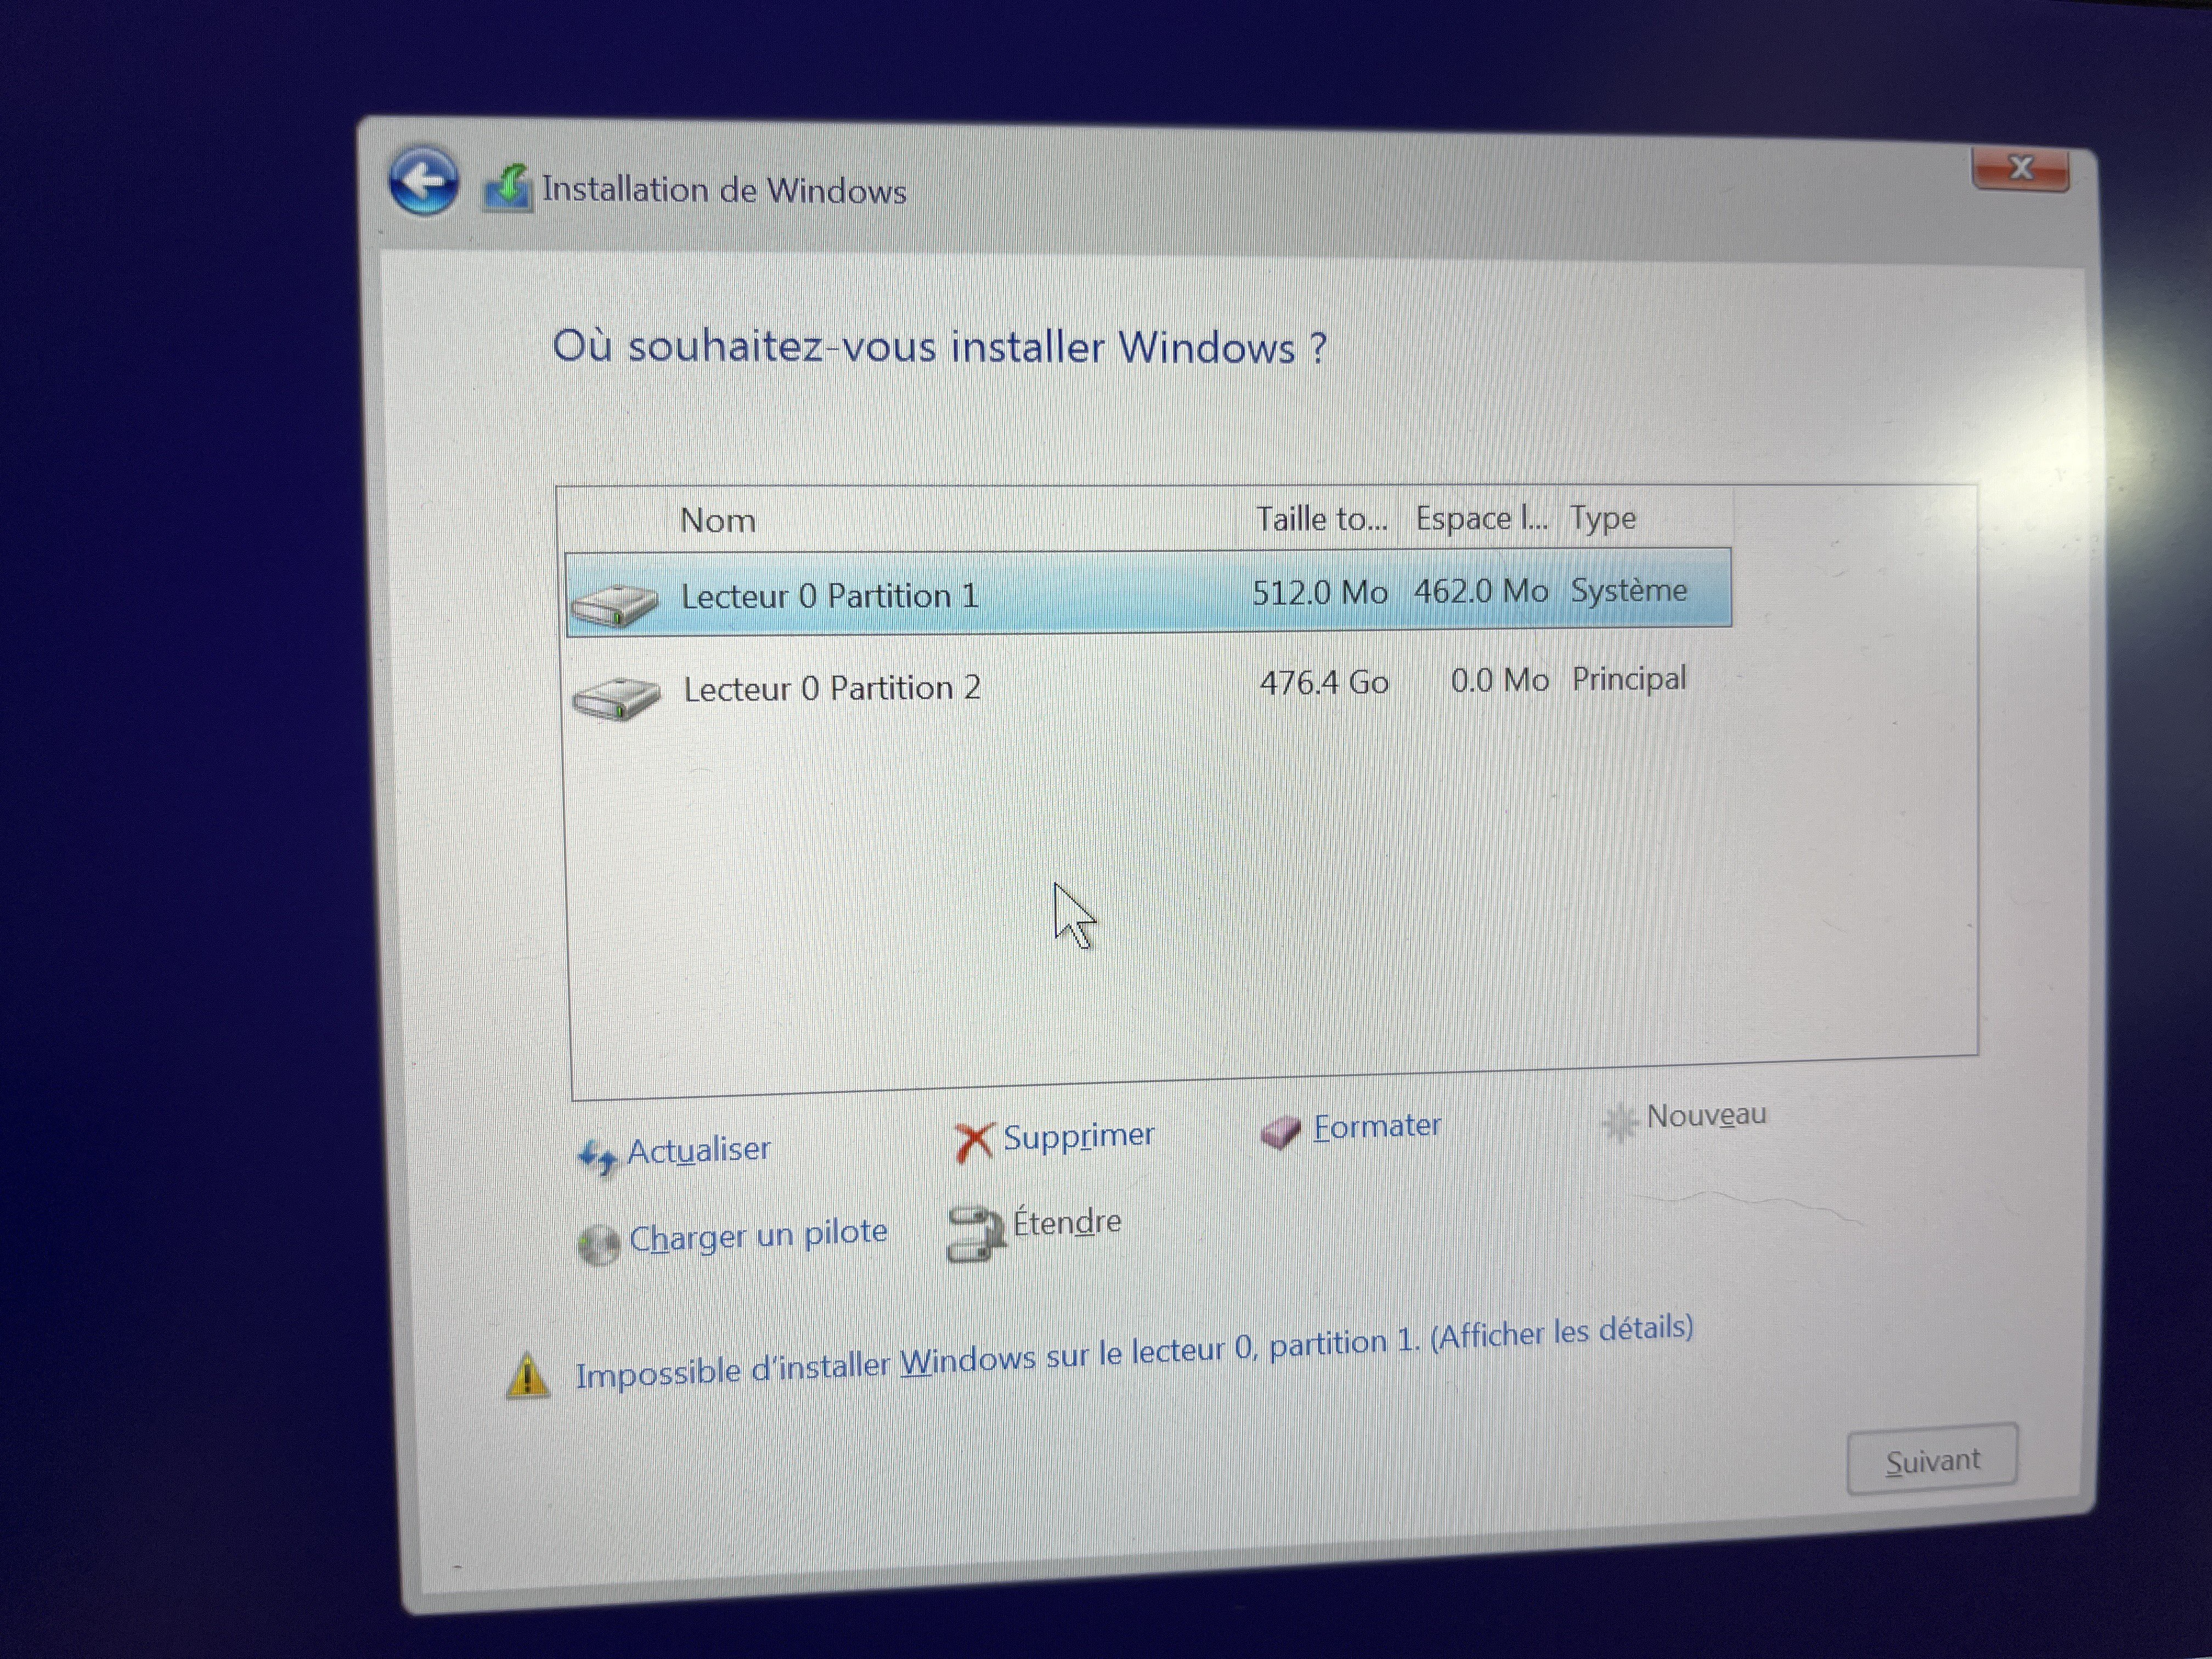
\includegraphics[width=0.7\textwidth]{disques.jpg}
  \caption{Ce qui devrait être normalement proposé si les options du \texttt{BIOS} sont OK}
  \label{fig:disquesOK}
\end{figure}
\section*{1. Cas classique}
\noindent Une fois votre clé \texttt{USB} créée, éteignez votre PC et accédez au \texttt{BIOS} (ou bien au \texttt{Boot Menu} pour les PCs plus récents) pour définir votre clé \texttt{USB} comme première option de démarrage. Selon le constructeur, checkez la \texttt{Table 1} pour voir la touche adéquate. Deux cas s'offrent à vous : 
\begin{itemize}
\item En cas d'accès au \texttt{Boot Menu} $\Rightarrow$ sélectionnez simplement votre clé USB avec les flèches directionnelles (haut et bas en l'occurrence) puis appuyez sur la touche \texttt{Entrée}. Laissez vous guider par l'installation de Windows jusqu'à l'étape disque (voir plus bas).
\item En cas d'accès au \texttt{BIOS} $\Rightarrow$ accédez au menu vous permettant de changer les options de démarrage (généralement : \texttt{Boot Options, HardDrive Disk Priority}, consultez sur Internet selon le constructeur de votre PC pour accéder à ce menu). Une fois trouvées, passez votre clé \texttt{USB} en première option de démarrage, quittez le \texttt{BIOS} en \textbf{ENREGISTRANT VOS MODIFICATIONS} (généralement touche \texttt{F10}). Laissez vous guider par l'installation de Windows jusqu'à l'étape disque (voir plus bas).
\end{itemize}
\noindent Une fois ces étapes \texttt{OK}, suivant les étapes d'installation de Windows 10 en vous laissant guider (faites bien \texttt{installation personnalisée} et non \texttt{mise à niveau} de Windows). Si tout est bien configuré sur votre PC et que les options du \texttt{BIOS} actuellement présentes vous permettent une installation correcte de Windows, vous devriez avoir quelque chose comme sur la \texttt{Figure 1} (\texttt{modulo} le nombre de disques que vous avez). Dans ce cas de figure : \textbf{SUPPRIMEZ UNE PAR UNE} les partitions de votre disque \texttt{SSD} utilisées (attention toutefois à ne pas supprimer les partitions de vos disques constituant vos données, comme un \texttt{HDD} interne par exemple), une fois toutes ces partitions supprimées, cliquez sur la partition où vous souhaitez installer Windows puis cliquez sur le bouton suivant (si le bouton n'est pas débloqué, créez une nouvelle partition avec l'espace libre créé juste avant, en prenant soin de laisser les options par défaut). Une fois cela fait, Windows devrait s'installer normalement sur votre machine. \\
\noindent \textbf{Remarque :} Windows ici devrait normalement repasser en première option de démarrage (cela dépend des \texttt{BIOS}), si vous ne redémarrez pas sur Windows au prochain démarrage, pensez à le remettre en première option de démarrage dans votre \texttt{BIOS} (voir \texttt{Figure 1} pour touches d'accès).
\section*{2. Cas pas classique}
\begin{figure}
  \begin{adjustwidth}{0cm}{}
    \begin{minipage}[t]{\textwidth}
      \centering
      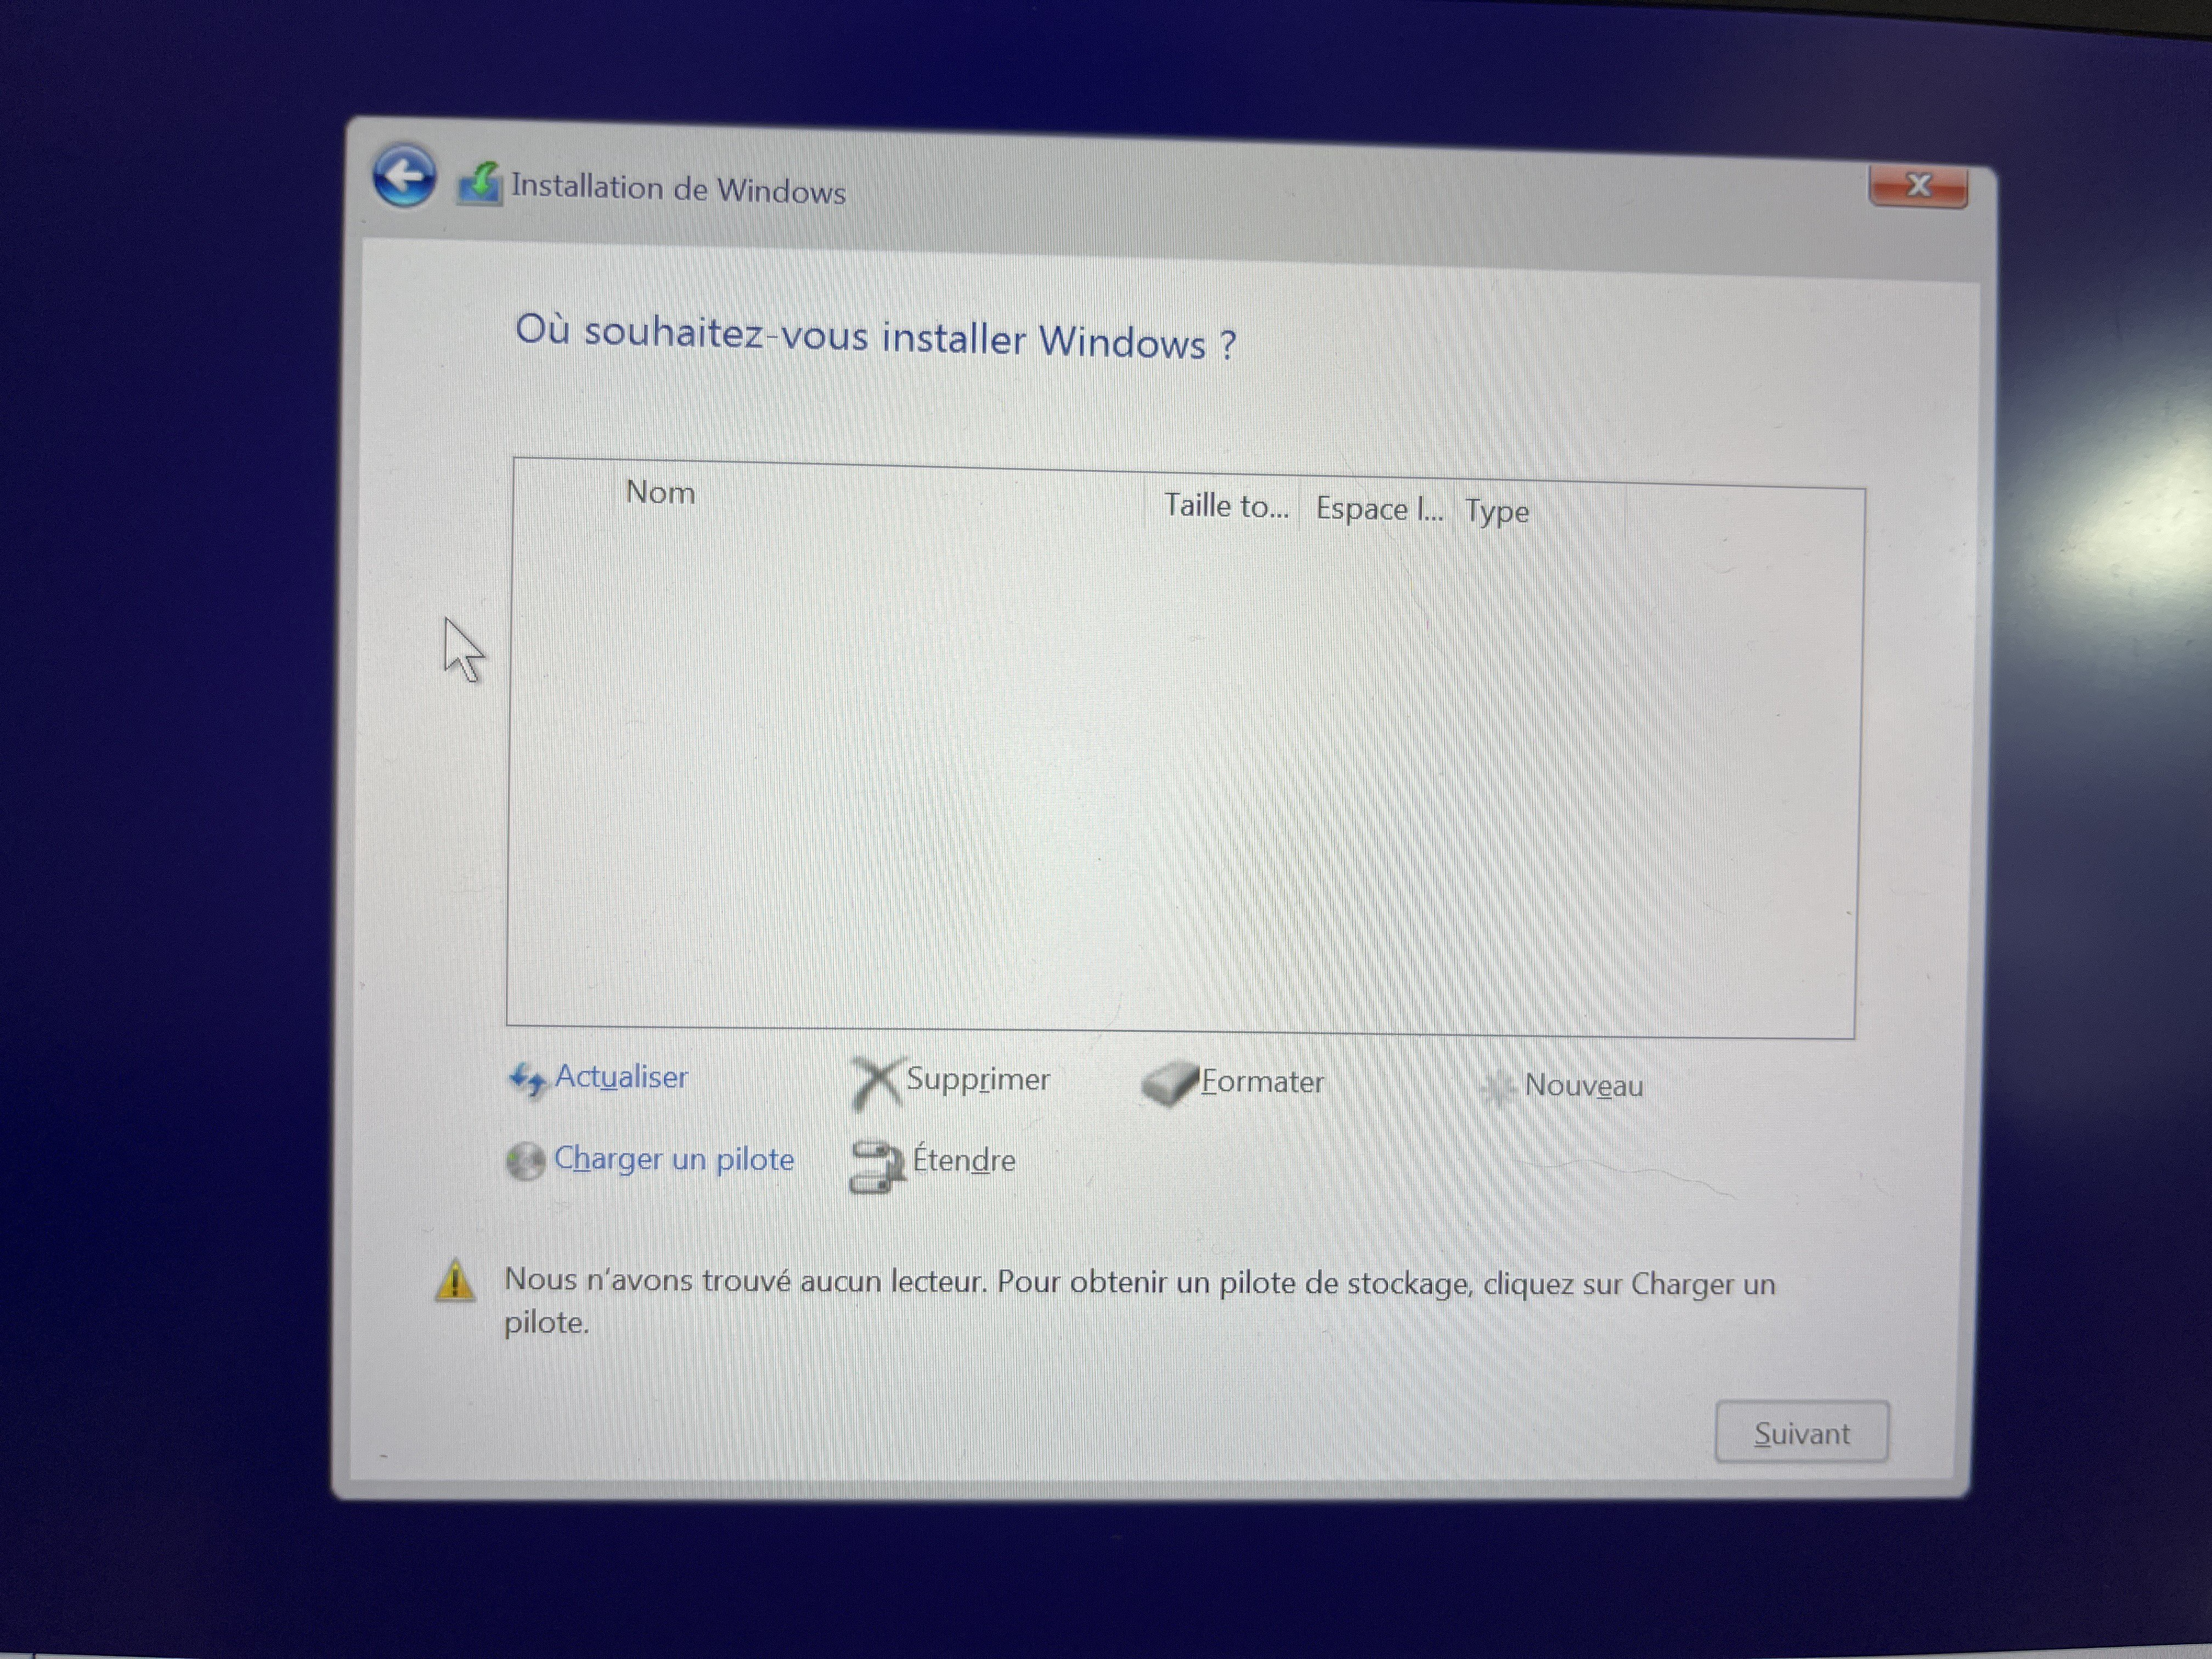
\includegraphics[width=0.43\textwidth]{pas_disques.jpg}\hspace{2cm}
      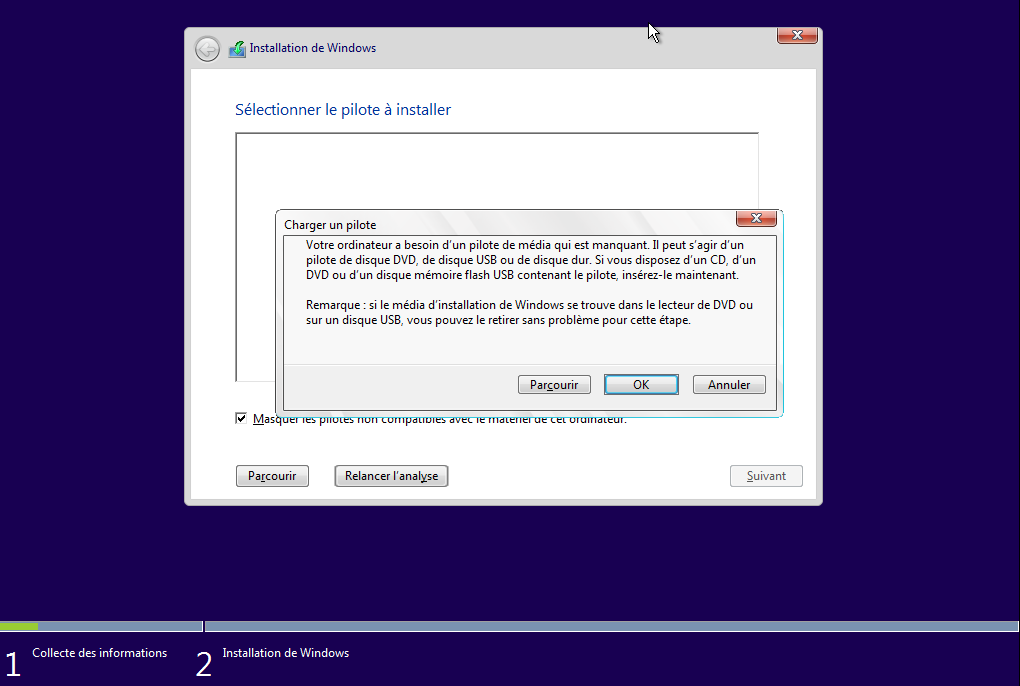
\includegraphics[width=0.43\textwidth]{no_pilots.png}
      \caption{Ce qui ne devrait pas être proposé}
      \label{fig:disquesPasOK}
    \end{minipage}
  \end{adjustwidth}
\end{figure}
\noindent Si en revanche vous avez l'un des deux cas qui s'affiche sur la \texttt{Figure 2}, c'est-à-dire qu'aucune des partitions de votre système n'est proposée, c'est qu'une option du \texttt{BIOS} nécessaire à l'installation de Windows n'est pas active, ou bien une option active ne devrait pas l'être. Il y a plusieurs explications possibles :
\begin{itemize}
\item Le \texttt{Secure Boot} est désactivé (dans ce cas $\Rightarrow$ ACTIVEZ LE ! Car il doit être activé pour l'installation de Windows, post-installation il peut être désactivé si vous le souhaitez, dans le cas d'un \texttt{dual boot} par exemple).
\item La clé USB n'a pas été configurée correctement (par exemple : mauvaise utilisation de l'outil \texttt{Ventoy}).
\item La clé \texttt{USB} que vous utilisez est corrompue (dans ce cas, essayez en une autre et voir si ça peut fonctionner). Dans la même idée, essayez de passer sur un port \texttt{USB 3} si votre clé était branchée sur un port \texttt{USB 2} (et inversement) pour voir si l'origine du problème est trouvée. Windows est particulièrement exigeant quant à l'installation du système, le moindre fichier manquant dans le media d'installation empêche l'installation du système et génère l'erreur de l'image de droite. Pour l'image de gauche, voir point suivant. 
\item Sur votre \texttt{BIOS}, le contrôleur de disques n'a pas la bonne définition (entre autre, pas la bonne option). Il existe plusieurs type de contrôleurs : \begin{itemize}
\item \texttt{RAID} $\Rightarrow$ plusieurs technologies de stockage utilisées à la fois avec différentes configurations
\item \texttt{AHCI} $\Rightarrow$ mode qui est apparu depuis les \texttt{SSD}, fonctionne grâce à la technologie \texttt{SATA} (native aux SSDs), accès plus rapide à la mémoire
\item \texttt{IDE} $\Rightarrow$ plus pour les anciens systèmes, remplacé par \texttt{SATA} depuis 2003. 	
\end{itemize}
Dans le cas d'une installation de Windows 10, on préfèrera généralement le mode \texttt{RAID} si vous disposez de plusieurs disques (plusieurs \texttt{HDD}, plusieurs \texttt{SSD}, ou bien \texttt{SSD + HDD}). Si vous ne disposez que d'un seul disque (ou plusieurs même disques) et qu'il s'agit d'un \texttt{SSD}, on préfèrera plutôt \texttt{AHCI}.
\item Il se peut qu'il manque un pilote (\texttt{RST Floppy}) dans le media d'installation de Windows, ce qui fait que le disque n'apparaît pas, voir \texttt{2.3} pour plus de précisions.
\end{itemize}
$ $\\ \noindent \textbf{Problème :} que faire ? quoi faire ? comment faire ? \\
\noindent \textbf{Remarque :} pour l'éventualité de changer la clé \texttt{USB} de port, le point ne sera pas abordé (problème plutôt trivial à gérer).\\
\subsection*{2.1 Première solution : activer le \texttt{Secure boot} dans le \texttt{BIOS}}
\begin{table}[ht]
    \centering
    \begin{tabular}{|c|>{\bfseries}c|}
        \hline
        \textbf{Constructeur} & \textbf{Emplacement dans le BIOS pour Secure Boot} \\
        \hline
        Acer & Boot $\rightarrow$ Secure Boot \\
        Apple & Non applicable \\
        ASUS & Boot $\rightarrow$ Secure Boot \\
        Dell & Boot $\rightarrow$ Secure Boot \\
        HP & Security $\rightarrow$ Secure Boot Configuration \\
        Lenovo & Security $\rightarrow$ Secure Boot \\
        MSI & Boot $\rightarrow$ Secure Boot \\
        Sony & Non applicable \\
        Toshiba & Advanced $\rightarrow$ Secure Boot \\
        \hline
    \end{tabular}
    \caption{Emplacement dans le \texttt{BIOS} pour vérifier le statut du \texttt{Secure boot} selon le constructeur. (Note: pour \texttt{Apple}, le \texttt{Secure boot} est géré automatiquement)}
    \label{tab:secure-boot-location}
\end{table}
\noindent De très loin la manipulation la plus simple, pour cela accédez à votre \texttt{BIOS} selon la touche du constructeur de votre PC (voir \texttt{Table 1} pour la touche). Une fois dans votre \texttt{BIOS}, vérifiez si le \texttt{Secure boot} est actif ou non selon l'endroit où se situe cette option (menus différents selon constructeurs). Ci-dessus, un tableau vous répertoriant dans quel menu vous devez vous rendre pour trouver cette option. Une fois l'option trouvée, vérifiez bien qu'elle est sur \texttt{ENABLED}, sinon passez-la en \texttt{ENABLED}. N'oubliez pas de sauvegarder vos modifications avant de quitter le \texttt{BIOS} !\\
\noindent Si elle était déjà en \texttt{ENABLED} mais que vos partitions n'apparaissaient pas, passez directement au \texttt{2.2}, sinon retentez une installation et voir si vos partitions apparaissent, en cas d'échec passez directement au \texttt{2.2}.
\subsection*{2.2 Seconde solution : regarder les options relatives au contrôleur de disques}
\begin{table}[ht]
    \centering
    \begin{tabular}{|c|>{\bfseries}c|}
        \hline
        \textbf{Constructeur} & \textbf{Emplacement dans le BIOS pour le contrôleur de disques} \\
        \hline
        Acer & Main $\rightarrow$ SATA Mode \\
        Apple & Non applicable \\
        ASUS & Advanced $\rightarrow$ SATA Configuration \\
        Dell & System Configuration $\rightarrow$ SATA Operation \\
        HP & Storage $\rightarrow$ Storage Options \\
        Lenovo & Config $\rightarrow$ Storage \\
        MSI & Integrated Peripherals $\rightarrow$ SATA Mode \\
        Sony & Non applicable \\
        Toshiba & Advanced $\rightarrow$ System Configuration $\rightarrow$ SATA Controller Mode \\
        \hline
    \end{tabular}
    \caption{Emplacement dans le \texttt{BIOS} pour changer le contrôleur de disques (\texttt{AHCI, RAID, IDE}) selon le constructeur.}
    \label{tab:sata-controller-location}
\end{table}
\noindent Ci-dessus, un tableau vous guidant sur comment trouver ce menu selon le constructeur de votre PC, cette option n'est pas forcément visible par défaut sur tous les \texttt{BIOS} (notamment HP), si vous ne trouvez pas nativement l'option, je vous invite à faire des recherches supplémentaires pour débloquer/trouver cette option dans votre \texttt{BIOS} (pour HP $\Rightarrow$ ce \href{https://h30434.www3.hp.com/t5/Notebook-Hardware-and-Upgrade-Questions/Cant-enable-AHCI-controller-mode-in-BIOS/td-p/7827723}{\color{blue} lien} pourra vous aider). Cette seconde solution est déjà un peu plus délicate, car on touche \textit{physiquement} à la configuration des disques. Avant toute chose, si vous avez des données dessus, pensez à en faire une sauvegarde, afin de ne rien perdre (juste une piqure de rappel classique, car même si on touche physiquement à la configuration des disques, les manipulations suivantes ne sont pas censées le corrompre, mais préférable par mesure de précaution). Si on en arrive là, mais que vous avez réussi à installer une distribution \texttt{Linux} (ou bien déjà installée), cela signifie qu'une option relative au contrôleur de vos disques a été modifiée (probablement par une mise à jour du \texttt{BIOS} post-installation de votre distribution \texttt{Linux}, ou bien avant). À partir de là, une fois le menu accédé, plusieurs options s'offrent à vous : 
\begin{itemize}
\item Si l'option était sur \texttt{AHCI ou IDE} $\rightarrow$ passez la sur \texttt{RAID}
\item Si l'option était sur \texttt{RAID ou IDE} $\rightarrow$ passez la sur \texttt{AHCI}
\end{itemize}
\begin{table}[ht]
    \centering
    \begin{tabular}{|c|>{\bfseries}c|}
        \hline
        \textbf{Constructeur} & \textbf{Emplacement dans le BIOS pour réinitialiser les réglages} \\
        \hline
        Acer & Exit $\rightarrow$ Load Setup Defaults \\
        Apple & Non applicable \\
        ASUS & Exit $\rightarrow$ Load Optimized Defaults \\
        Dell & Exit $\rightarrow$ Load Defaults \\
        HP & File $\rightarrow$ Default Setup \\
        Lenovo & Exit $\rightarrow$ Load Default Settings \\
        MSI & Save \& Exit $\rightarrow$ Restore Defaults \\
        Sony & Non applicable \\
        Toshiba & Exit $\rightarrow$ Load Setup Defaults \\
        \hline
    \end{tabular}
    \caption{Emplacement dans le \texttt{BIOS} pour réinitialiser les réglages par défaut selon le constructeur.}
    \label{tab:reset-bios-location}
\end{table}
\noindent \textbf{Remarque :} sur Windows, le mode \texttt{AHCI} est préféré (pour détection des disques à l'installation).\\
\textbf{Remarque :} comme on suppose que votre PC est plus ou moins récent (à partir de 2018 on peut le considérer comme récent), on ne préfèrera pas mettre l'option \texttt{IDE}.\\
\noindent À partir de là, sauvegardez vos modifications, quittez votre \texttt{BIOS} et retentez une installation pour voir si cette fois-ci vos partitions sont bien détectées (au même titre que sur la \texttt{Figure 1}). Si suite à cela l'installation est toujours en échec, revenez dans votre \texttt{BIOS} et \textbf{réinitialisez les réglages par défaut}. Ci-dessus, un tableau vous répertoriant selon le constructeur de votre PC comment effectuer cette opération (ce que ça fera surtout : activation du \texttt{Secure boot}, paramétrage des disques remis par défaut, car on ne sait guère ce qui peut déclencher un blocage de la sorte, donc autant réinitialiser les réglages par solution de facilité). \\
\noindent Une fois cela fait, retentez une installation de Windows, elle devrait être cette fois-ci fructueuse. Dans le cas d'une installation toujours infructueuse, deux options s'offrent à vous : 
\begin{itemize}
\item Dans le cas de l'image de droite de la \texttt{Figure 2}, passez directement au \texttt{2.3}.
\item Sinon, si et seulement si vous avez bien suivi toutes les étapes ci-dessus, et que l'installation est toujours infructueuse, alors contactez moi sur discord, soit en privé en m'ajoutant en ami : \texttt{naelebk}, soit en rejoignant mon \href{https://discord.gg/ja7t6Aq}{\color{blue} serveur discord}.
\end{itemize}
\subsection*{2.3 Troisième solution : ajouter un pilote additionnel dans votre media d'installation}
\begin{table}[ht]
    \centering
    \begin{tabular}{|c|c|}
        \hline
        \textbf{Constructeur} & \textbf{Installation des Pilotes} \\
        \hline
        Intel + AMD & Téléchargez les pilotes depuis le site officiel d'Intel (\href{https://www.intel.fr/content/www/fr/fr/download/771902/intel-rapid-storage-technology-intel-rst-driver-for-windows-10-64-bit-windows-11-for-intel-nuc-11-enthusiast-kit-mini-pc-nuc11phki7.html}{\color{blue} first link}). \\
        \hline
    \end{tabular}
    \caption{Installation des pilotes pour processeurs Intel et AMD.}
    \label{tab:install-pilotes}
\end{table}

\noindent Comme il n'existe que deux types de processeur (\texttt{Intel} et \texttt{AMD}), l'installation des pilotes se fera plutôt facilement, car mêmes pilotes dans un cas et dans l'autre. Ci-dessus, un tableau vous récapitulant le lien d'installation des pilotes. Dans un cas ou dans l'autre, après téléchargement du fichier \texttt{ZIP} correspondant, il faut extraire le \texttt{ZIP} \textbf{DANS} votre clé USB d'installation Windows, ce qui permettra, au moment d'arriver à la \texttt{Figure 2}, de charger directement le pilote en sélectionnant le répertoire correspondant (ou bien exécuter le programme correspondant). Cette fois-ci, l'installation \textit{doit} être fructueuse.
\end{document}